\documentclass{article}
\usepackage{graphicx} % Required for inserting images
\usepackage[top=0.9in, bottom=1in, left=1.5in, right=1.5in]{geometry}
\usepackage[utf8]{inputenc}
\usepackage[icelandic]{babel}
\usepackage[T1]{fontenc}
\usepackage[sc]{mathpazo}
\usepackage[parfill]{parskip}
\renewcommand{\baselinestretch}{1.2}
% Tables and lists
\usepackage{booktabs,tabularx}
\usepackage{multirow}
\usepackage{enumerate}
\usepackage{adjustbox}
\usepackage{multicol}
\usepackage{xcolor}
\usepackage{algpseudocode}
\usepackage{tikz}
\usepackage{nicefrac}
\usepackage{changepage}
\usetikzlibrary{arrows, positioning, calc, graphs}

% Math
\usepackage{amsmath, amsfonts, amssymb, amsthm}
% Graphics

\usepackage{graphicx}
\usepackage{tikz}
% Code environment
\usepackage{minted}
%\usepackage{bm}
%\usepackage{siunitx}
%\usepackage{animate}
%\usepackage{hyperref}
%\usepackage{movie15}
%\usepackage{multicol}
%\usepackage{changepage}
\title{Formal Languages and Computability 3}
\author{Ragnar Björn Ingvarsson, rbi3}
\tikzset{->, >=stealth', shorten >=1pt, node distance=2cm,thick, main node/.style={circle,draw,minimum size=3em}}


\begin{document}
\renewcommand\thepage{}
	
	\maketitle

	\newpage
	\setcounter{page}{1}
	\renewcommand\thepage{\arabic{page}}
	\section{Let us consider the language $L(00^*(0\cup 1))$}

	\begin{itemize}
		\item[a)] \textbf{Draw the state diagram of an NFA that 
			accepts it.}

			\begin{center}
			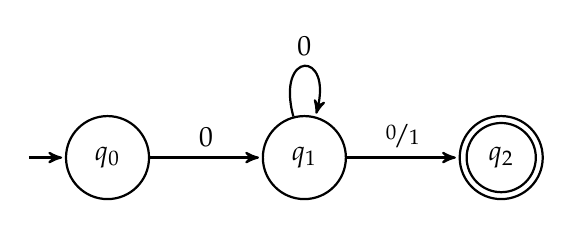
\begin{tikzpicture}[thick,auto]
				\node[main node] (q0) {$q_0$};
				\node[main node] at (2.5,0) (q1) {$q_1$};
				\node[main node] at (5,0) (q2) {$q_2$};
				\node[main node, minimum size=2.5em] at (5,0) (q2fin) {};

				\path (-1,0) edge node {} (q0);
				\path (q0) edge node {0} (q1);
				\path (q1) edge[loop above=20] node {0} (q1);
				\path (q1) edge node {$\nicefrac{0}{1}$} (q2);
			\end{tikzpicture}
			\end{center}
		\item[b)] \textbf{Convert the NFA to a simple RE.}

			We add states $q_s$ and $q_f$ and add an epsilon 
			transition from $q_s$ to the start state and an epsilon 
			transition from each finish state to $q_f$, changing 
			each finish state to a normal state and making $q_f$ 
			the only finish state, and get

			\begin{center}
				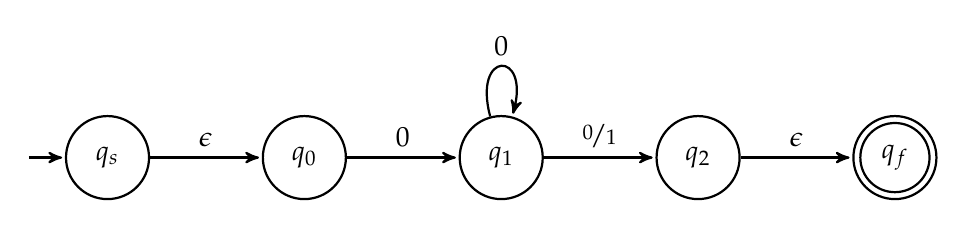
\begin{tikzpicture}[thick,auto]
				\node[main node] at (-2.5,0) (qs) {$q_s$};
				\node[main node] (q0) {$q_0$};
				\node[main node] at (2.5,0) (q1) {$q_1$};
				\node[main node] at (5,0) (q2) {$q_2$};
				\node[main node] at (7.5,0) (qf) {$q_f$};
				\node[main node, minimum size=2.5em] at (7.5,0) (qffin) {};

				\path (-3.5,0) edge node {} (qs);
				\path (q0) edge node {0} (q1);
				\path (q1) edge[loop above=20] node {0} (q1);
				\path (q1) edge node {$\nicefrac{0}{1}$} (q2);
				\path (qs) edge node {$\epsilon$} (q0);
				\path (q2) edge node {$\epsilon$} (qf);
				\end{tikzpicture}
			\end{center}

			And we simplify, eliminating firstly the loop on $q_1$:

			\begin{center}
				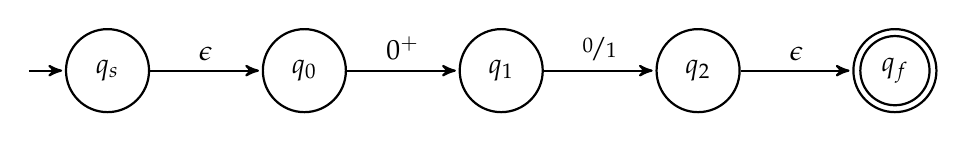
\begin{tikzpicture}[thick,auto]
				\node[main node] at (-2.5,0) (qs) {$q_s$};
				\node[main node] (q0) {$q_0$};
				\node[main node] at (2.5,0) (q1) {$q_1$};
				\node[main node] at (5,0) (q2) {$q_2$};
				\node[main node] at (7.5,0) (qf) {$q_f$};
				\node[main node, minimum size=2.5em] at (7.5,0) (qffin) {};

				\path (-3.5,0) edge node {} (qs);
				\path (q0) edge node {$0^+$} (q1);
				\path (q1) edge node {$\nicefrac{0}{1}$} (q2);
				\path (qs) edge node {$\epsilon$} (q0);
				\path (q2) edge node {$\epsilon$} (qf);
				\end{tikzpicture}
			\end{center}

			And then eliminating state $q_1$:

			\begin{center}
				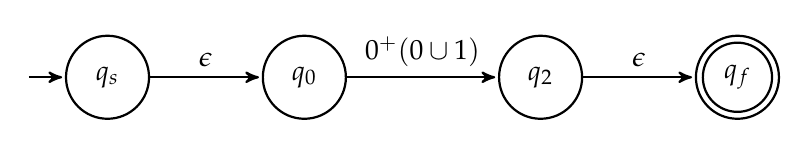
\begin{tikzpicture}[thick,auto]
				\node[main node] at (-2.5,0) (qs) {$q_s$};
				\node[main node] (q0) {$q_0$};
				\node[main node] at (3,0) (q2) {$q_2$};
				\node[main node] at (5.5,0) (qf) {$q_f$};
				\node[main node, minimum size=2.5em] at (5.5,0) (qffin) {};

				\path (-3.5,0) edge node {} (qs);
				\path (q0) edge node {$0^+(0\cup 1)$} (q2);
				\path (qs) edge node {$\epsilon$} (q0);
				\path (q2) edge node {$\epsilon$} (qf);
				\end{tikzpicture}
			\end{center}

			And now we have simplified the NFA and we get the 
			regular expression $0^+(0\cup 1)$.

	\end{itemize}

	\newpage
	\section{Suppose the input alphabet is binary numbers, $\Sigma 
		= \{0,1\}$, and language $A$ consists of binary numbers $x$ 
		such that $x \text{ mod } 3 = 1$. Determine a regular expression for 
	$A$.}

	We can start from making a DFA describing the language:

	\begin{center}
	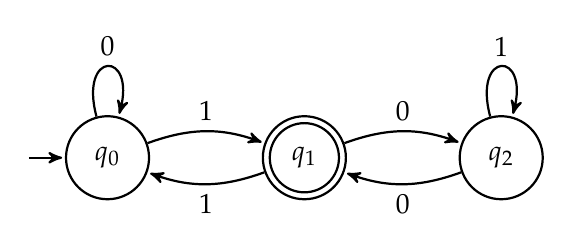
\begin{tikzpicture}[thick,auto]
		\node[main node] (q0) {$q_0$};
		\node[main node] at (2.5,0) (q1) {$q_1$};
		\node[main node, minimum size=2.5em] at (2.5,0) (q1fin) {};
		\node[main node] at (5,0) (q2) {$q_2$};

		\path (-1,0) edge node {} (q0);
		\path (q0) edge[loop above=20] node {0} (q0);
		\path (q0) edge[bend left=20] node {1} (q1);
		\path (q1) edge[bend left=20] node {1} (q0);
		\path (q1) edge[bend left=20] node {0} (q2);
		\path (q2) edge[bend left=20] node {0} (q1);
		\path (q2) edge[loop above=20] node {1} (q2);
	\end{tikzpicture}
	\end{center}

	And then start converting to a regular expression:

	\begin{center}
	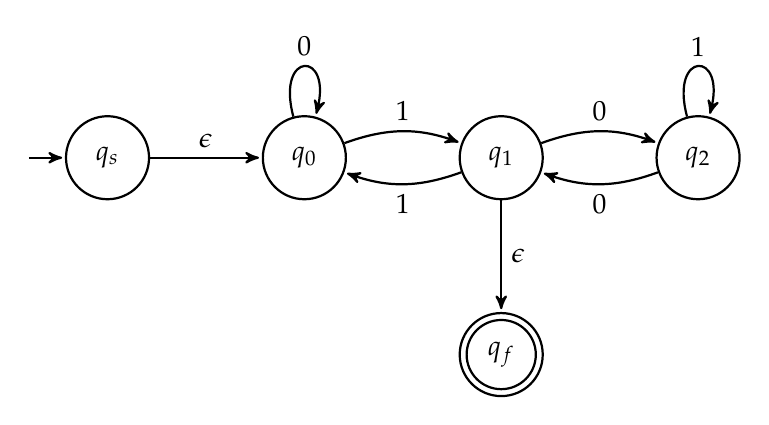
\begin{tikzpicture}[thick,auto]
		\node[main node] at (-2.5,0) (qs) {$q_s$};
		\node[main node] (q0) {$q_0$};
		\node[main node] at (2.5,0) (q1) {$q_1$};
		\node[main node] at (5,0) (q2) {$q_2$};
		\node[main node] at (2.5,-2.5) (qf) {$q_f$};
		\node[main node, minimum size=2.5em] at (2.5,-2.5) (qffin) {};

		\path (-3.5,0) edge node {} (qs);
		\path (qs) edge node {$\epsilon$} (q0);
		\path (q0) edge[loop above=20] node {0} (q0);
		\path (q0) edge[bend left=20] node {1} (q1);
		\path (q1) edge[bend left=20] node {1} (q0);
		\path (q1) edge[bend left=20] node {0} (q2);
		\path (q2) edge[bend left=20] node {0} (q1);
		\path (q2) edge[loop above=20] node {1} (q2);
		\path (q1) edge node {$\epsilon$} (qf);
	\end{tikzpicture}
	\end{center}

	Where from we can simplify the path between $q_0$ and $q_1$:

	\begin{center}
	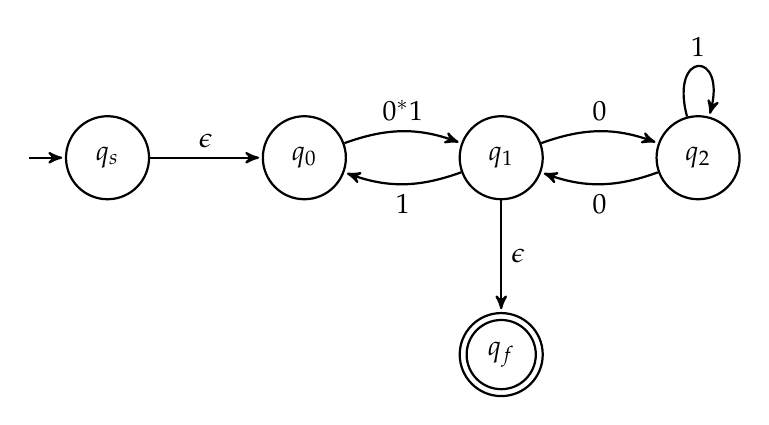
\begin{tikzpicture}[thick,auto]
		\node[main node] at (-2.5,0) (qs) {$q_s$};
		\node[main node] (q0) {$q_0$};
		\node[main node] at (2.5,0) (q1) {$q_1$};
		\node[main node] at (5,0) (q2) {$q_2$};
		\node[main node] at (2.5,-2.5) (qf) {$q_f$};
		\node[main node, minimum size=2.5em] at (2.5,-2.5) (qffin) {};

		\path (-3.5,0) edge node {} (qs);
		\path (qs) edge node {$\epsilon$} (q0);
		\path (q0) edge[bend left=20] node {$0^*1$} (q1);
		\path (q1) edge[bend left=20] node {1} (q0);
		\path (q1) edge[bend left=20] node {0} (q2);
		\path (q2) edge[bend left=20] node {0} (q1);
		\path (q2) edge[loop above=20] node {1} (q2);
		\path (q1) edge node {$\epsilon$} (qf);
	\end{tikzpicture}
	\end{center}

	And then we can remove the path from $q_1$ to $q_0$:

\begin{center}
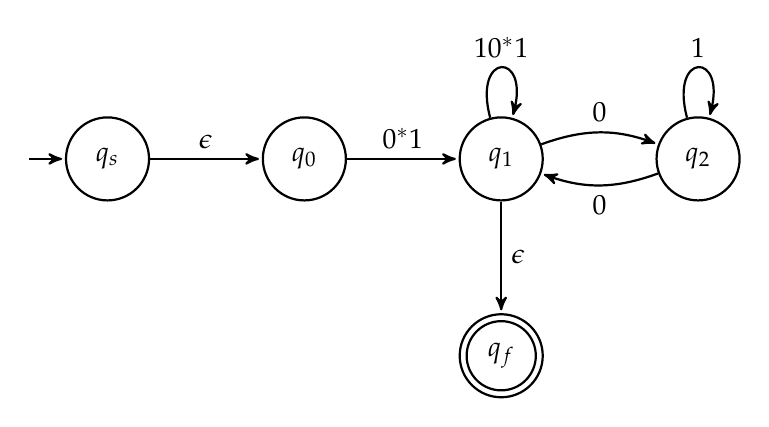
\begin{tikzpicture}[thick,auto]
	\node[main node] at (-2.5,0) (qs) {$q_s$};
	\node[main node] (q0) {$q_0$};
	\node[main node] at (2.5,0) (q1) {$q_1$};
	\node[main node] at (5,0) (q2) {$q_2$};
	\node[main node] at (2.5,-2.5) (qf) {$q_f$};
	\node[main node, minimum size=2.5em] at (2.5,-2.5) (qffin) {};

	\path (-3.5,0) edge node {} (qs);
	\path (qs) edge node {$\epsilon$} (q0);
	\path (q0) edge node {$0^*1$} (q1);
	\path (q1) edge[loop above=20] node {$10^*1$} (q1);
	\path (q1) edge[bend left=20] node {0} (q2);
	\path (q2) edge[bend left=20] node {0} (q1);
	\path (q2) edge[loop above=20] node {1} (q2);
	\path (q1) edge node {$\epsilon$} (qf);
\end{tikzpicture}
\end{center}

Finally we do the same for $q_2$ and get:

\begin{center}
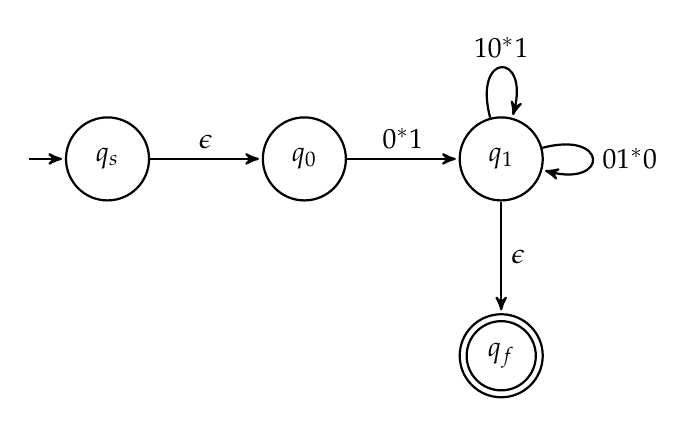
\begin{tikzpicture}[thick,auto]
	\node[main node] at (-2.5,0) (qs) {$q_s$};
	\node[main node] (q0) {$q_0$};
	\node[main node] at (2.5,0) (q1) {$q_1$};
	\node[main node] at (2.5,-2.5) (qf) {$q_f$};
	\node[main node, minimum size=2.5em] at (2.5,-2.5) (qffin) {};

	\path (-3.5,0) edge node {} (qs);
	\path (qs) edge node {$\epsilon$} (q0);
	\path (q0) edge node {$0^*1$} (q1);
	\path (q1) edge[loop above=20] node {$10^*1$} (q1);
	\path (q1) edge[loop right=20] node {$01^*0$} (q1);
	\path (q1) edge node {$\epsilon$} (qf);
\end{tikzpicture}
\end{center}

Then combine everything into a single path:

\begin{center}
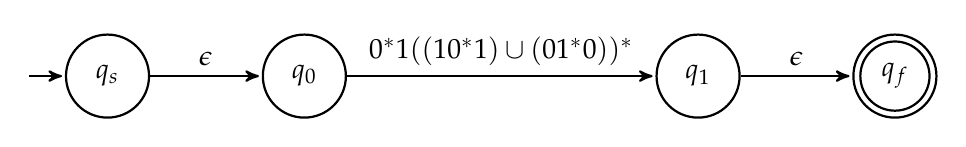
\begin{tikzpicture}[thick,auto]
	\node[main node] at (-2.5,0) (qs) {$q_s$};
	\node[main node] (q0) {$q_0$};
	\node[main node] at (5,0) (q1) {$q_1$};
	\node[main node] at (7.5,0) (qf) {$q_f$};
	\node[main node, minimum size=2.5em] at (7.5,0) (qffin) {};

	\path (-3.5,0) edge node {} (qs);
	\path (qs) edge node {$\epsilon$} (q0);
	\path (q0) edge node {$0^*1((10^*1)\cup (01^*0))^*$} (q1);
	\path (q1) edge node {$\epsilon$} (qf);
\end{tikzpicture}
\end{center}

So the regular expression is $0^*1((10^*1)\cup(01^*0))^*$.

\newpage
\section{Let $\Sigma = {a,...,t}$ denote the numbers $0,...,19$ in 
	that order. Let $A$ denote the language that consists of all strings 
whose numerical value is less than 42. Determine a regular expression 
for $A$.}

We notice here that the string can start with an undetermined 
amount of $a$'s (0's), and after that we have three cases:

\begin{itemize}
	\item Any letter in the alphabet with nothing to follow, $0-19$.
	\item $b$, followed then by any letter in the alphabet, $20-39$.
	\item $c$, followed exclusively by either one $a$ or one $b$, 
		$40-41$.
\end{itemize}

We can then write out the regular expression:
\[a^*((b\Sigma)\cup(c(a\cup b))\cup\Sigma)\]

Here we have also excluded the possibility of the empty string since 
it does not have a numerical value.

\newpage
\section{Let us continue with the Mayan numbers. Let language $A$ consist of numbers $x$ such that $x 
\text{ mod } 3 = 1$.}

\begin{itemize}
	\item[a)] \textbf{Determine a DFA that recognizes $A$.}

		Let us divide the alphabet $\Sigma$ into three subsets, 
		\begin{itemize}
			\item $\Sigma_0 = \{x\in \Sigma | x \text{ mod }3 = 0\}$
			\item $\Sigma_1 = \{x\in \Sigma | x \text{ mod }3 = 1\}$
			\item $\Sigma_2 = \{x\in \Sigma | x \text{ mod }3 = 2\}$
		\end{itemize}

		And then notice that since we are multiplying by $20$ with 
		each letter added, if we research what happens only if we 
		add $a$, we get that from a remainder of $0$, we get 
		a remainder of $0*20\text{ mod }3 = 0$, from $1$ we get 
		$1*20\text{ mod }3 = 2$ and from $2$ we get 
		$2*20\text{ mod }3 = 1$.

		That leads to this DFA:

		\begin{center}
		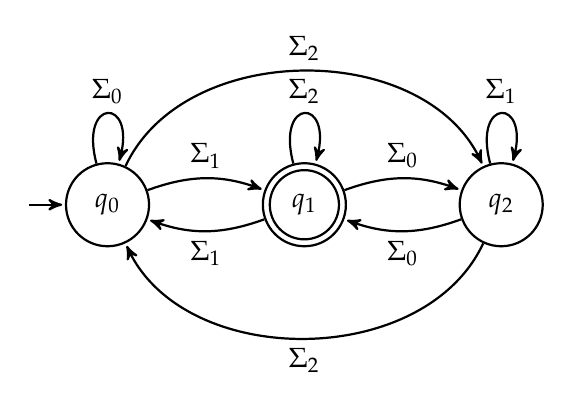
\begin{tikzpicture}[thick,auto]
			\node[main node] (q0) {$q_0$};
			\node[main node] at (2.5,0) (q1) {$q_1$};
			\node[main node,minimum size=2.5em] at (2.5,0) (q1fin) {};
			\node[main node] at (5,0) (q2) {$q_2$};

			\path (-1,0) edge node {} (q0);
			\path (q0) edge[loop above=20] node {$\Sigma_0$} (q0);
			\path (q1) edge[loop above=20] node {$\Sigma_2$} (q1);
			\path (q2) edge[loop above=20] node {$\Sigma_1$} (q2);
			\path (q0) edge[bend left=20] node {$\Sigma_1$} (q1);
			\path (q1) edge[bend left=20] node {$\Sigma_1$} (q0);
			\path (q1) edge[bend left=20] node {$\Sigma_0$} (q2);
			\path (q2) edge[bend left=20] node {$\Sigma_0$} (q1);
			\path (q0) edge[bend left=65] node {$\Sigma_2$} (q2);
			\path (q2) edge[bend left=65] node {$\Sigma_2$} (q0);
		\end{tikzpicture}
		\end{center}
	\item[b)] \textbf{Give a regular expression for $A$.}

		We use the DFA in a) and convert it to a regular expression, 
		and so we begin with this:

		\begin{center}
		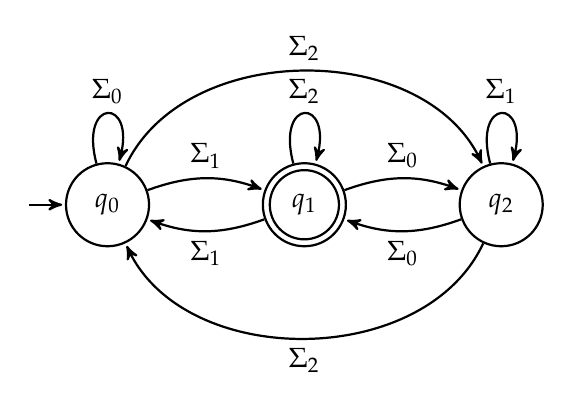
\begin{tikzpicture}[thick,auto]
			\node[main node] (q0) {$q_0$};
			\node[main node] at (2.5,0) (q1) {$q_1$};
			\node[main node,minimum size=2.5em] at (2.5,0) (q1fin) {};
			\node[main node] at (5,0) (q2) {$q_2$};

			\path (-1,0) edge node {} (q0);
			\path (q0) edge[loop above=20] node {$\Sigma_0$} (q0);
			\path (q1) edge[loop above=20] node {$\Sigma_2$} (q1);
			\path (q2) edge[loop above=20] node {$\Sigma_1$} (q2);
			\path (q0) edge[bend left=20] node {$\Sigma_1$} (q1);
			\path (q1) edge[bend left=20] node {$\Sigma_1$} (q0);
			\path (q1) edge[bend left=20] node {$\Sigma_0$} (q2);
			\path (q2) edge[bend left=20] node {$\Sigma_0$} (q1);
			\path (q0) edge[bend left=65] node {$\Sigma_2$} (q2);
			\path (q2) edge[bend left=65] node {$\Sigma_2$} (q0);
		\end{tikzpicture}
		\end{center}

		From where we want to eliminate $q_2$ by using the state 
		elimination method:
		
		\begin{center}
		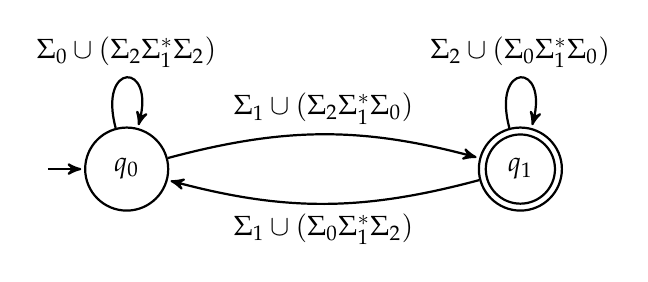
\begin{tikzpicture}[thick,auto]
			\node[main node] (q0) {$q_0$};
			\node[main node] at (5,0) (q1) {$q_1$};
			\node[main node,minimum size=2.5em] at (5,0) (q1fin) {};

			\path (-1,0) edge node {} (q0);
			\path (q0) edge[loop above=20] node {$
			\Sigma_0\cup(\Sigma_2\Sigma_1^*\Sigma_2)$} (q0);
			\path (q1) edge[loop above=20] node {$
			\Sigma_2\cup(\Sigma_0\Sigma_1^*\Sigma_0)$} (q1);
			\path (q0) edge[bend left=15] node {$
			\Sigma_1\cup(\Sigma_2\Sigma_1^*\Sigma_0)$} (q1);
			\path (q1) edge[bend left=15] node {$
			\Sigma_1\cup(\Sigma_0\Sigma_1^*\Sigma_2)$} (q0);
		\end{tikzpicture}
		\end{center}

		Now we remove the loops:

		\begin{center}
		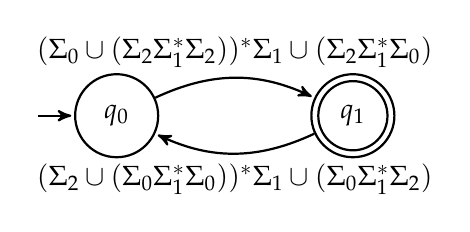
\begin{tikzpicture}[thick,auto]
			\node[main node] (q0) {$q_0$};
			\node[main node] at (3,0) (q1) {$q_1$};
			\node[main node,minimum size=2.5em] at (3,0) (q1fin) {};

			\path (-1,0) edge node {} (q0);
			\path (q0) edge[bend left=25] node {$
				(\Sigma_0\cup(\Sigma_2\Sigma_1^*\Sigma_2))^*
				\Sigma_1\cup(\Sigma_2\Sigma_1^*\Sigma_0)
			$} (q1);
			\path (q1) edge[bend left=25] node {$
				(\Sigma_2\cup(\Sigma_0\Sigma_1^*\Sigma_0))^*
			\Sigma_1\cup(\Sigma_0\Sigma_1^*\Sigma_2)
		$} (q0);
		\end{tikzpicture}
		\end{center}

		And now, for simplification, we can say that the transition 
		from $q_0$ to $q_1$ is $\alpha$ and from $q_1$ to $q_0$ is 
		$\beta$, and we get

		\begin{center}
		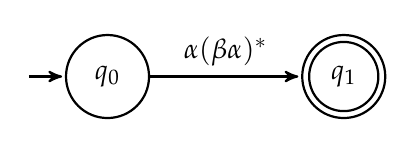
\begin{tikzpicture}[thick,auto]
			\node[main node] (q0) {$q_0$};
			\node[main node] at (3,0) (q1) {$q_1$};
			\node[main node,minimum size=2.5em] at (3,0) (q1fin) {};

			\path (-1,0) edge node {} (q0);
			\path (q0) edge node {$\alpha(\beta\alpha)^*$} (q1);
		\end{tikzpicture}
		\end{center}

		And that is the regular expression, $\alpha(\beta\alpha)^*$, 
		or in its entirety:

		\begin{adjustwidth}{-100pt}{-100pt}
				\[(\Sigma_0\cup(\Sigma_2\Sigma_1^*\Sigma_2))^*
				\Sigma_1\cup(\Sigma_2\Sigma_1^*\Sigma_0)
				((\Sigma_2\cup(\Sigma_0\Sigma_1^*\Sigma_0))^*
			\Sigma_1\cup(\Sigma_0\Sigma_1^*\Sigma_2)
				(\Sigma_0\cup(\Sigma_2\Sigma_1^*\Sigma_2))^*
			\Sigma_1\cup(\Sigma_2\Sigma_1^*\Sigma_0))^*\]
		\end{adjustwidth}


\end{itemize}

\end{document}
